\chapter{Joint Inversion}\label{Chp:cook:joint inversion}

A striking interpretation of a joint inversion 3D model of gravity and magnetic data could solve a big problem of exploration geophysics. Traditionally inversion of magnetic and gravity data provide a 3D physical rock property model separately. However the inversion different type of datasets could supplement the result. In the meantime joint inversion by making more constraints on characteristics modify the outcome.

In this section a new package is significantly presented to provide a joint model of density and magnetic susceptibility which undertake an apparent discrepancy in terms of geophysical approach. This package is based on geological smooth model in density and magnetic susceptibility variations. There is an example with real data on gravity and magnetic anomalies with result on density and susceptibility.(\ref{fig:jointden1}, \ref{fig:jointden11}, \ref{fig:jointsus1} and \ref{fig:jointsus2})


% \begin{figure}
% \centering
% 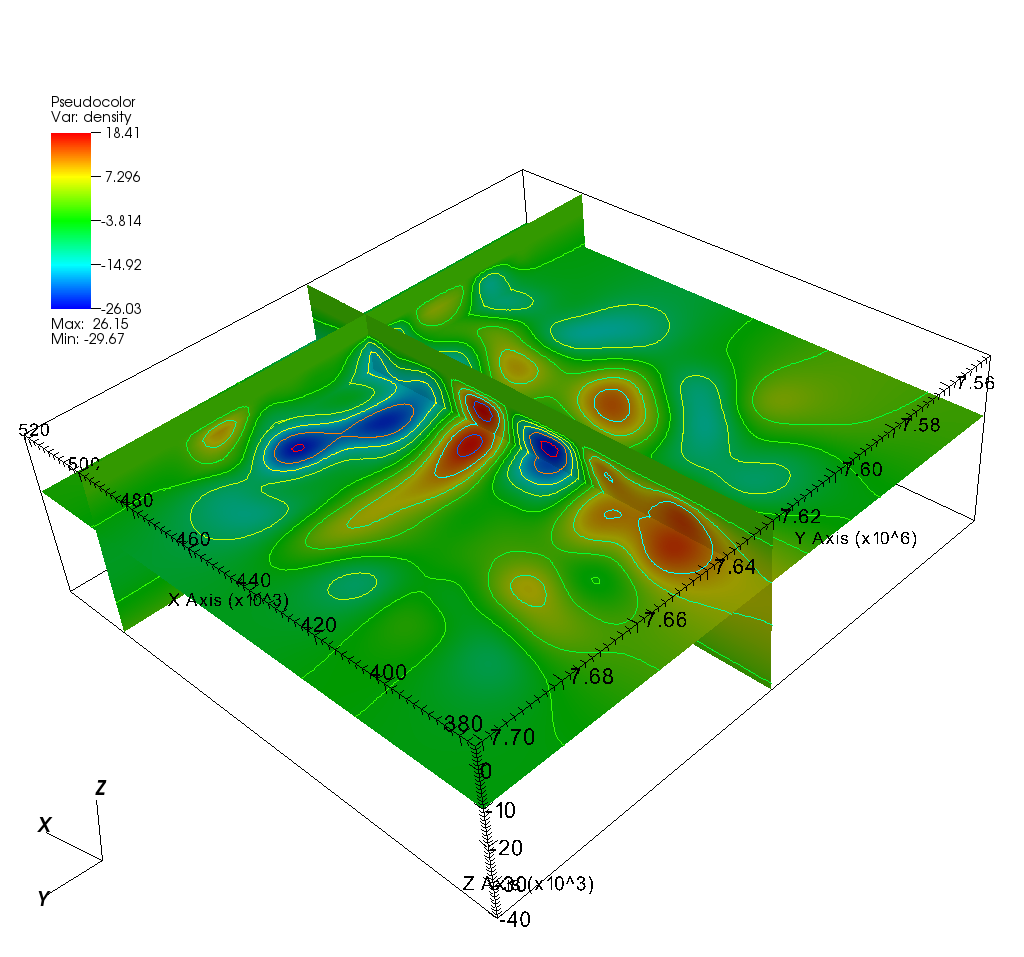
\includegraphics[width=\textwidth]{jointden1.png}
% \caption{3D map on density result in joint inversion with two cross and a depth section}
% \label{fig:jointden1}
% \end{figure}
% 
% 
% \begin{figure}
% \centering
% 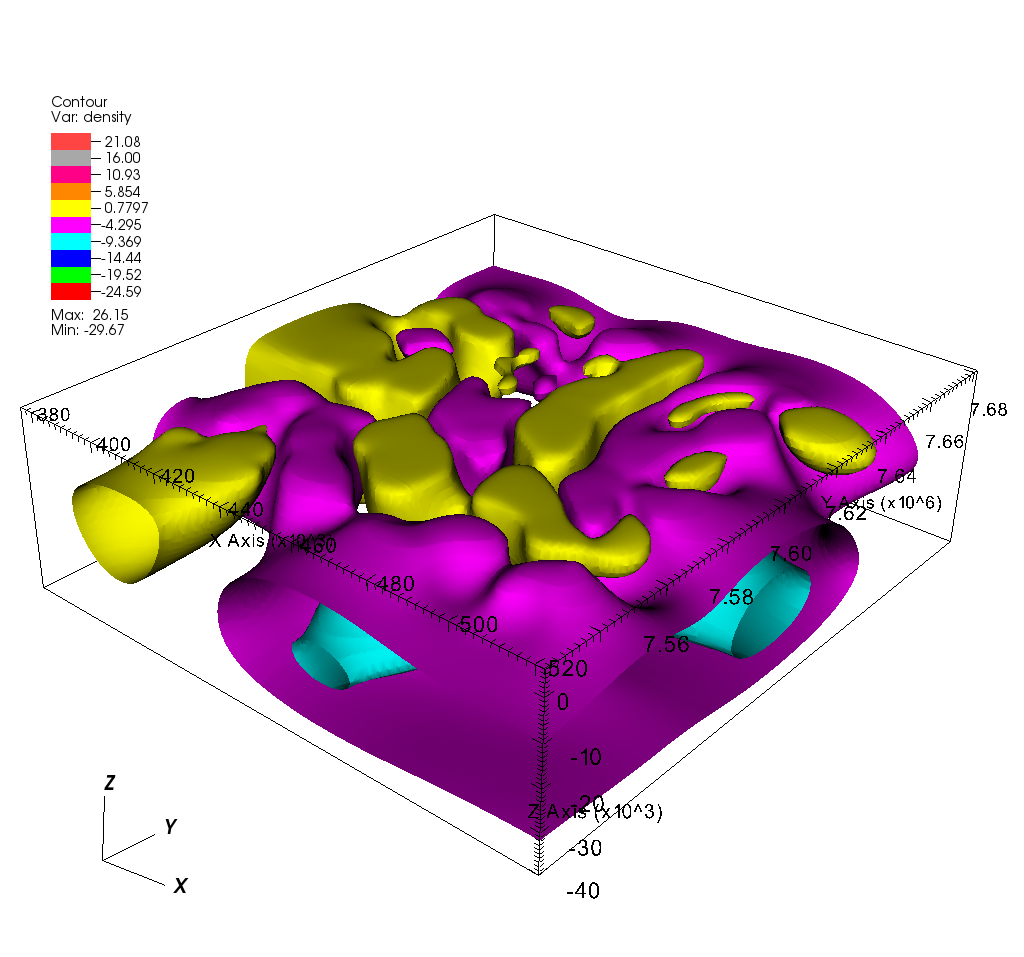
\includegraphics[width=\textwidth]{jointden11.png}
% \caption{3D contour map on density result in joint inversion }
% \label{fig:jointden11}
% \end{figure}
% 
% \begin{figure}
% \centering
% 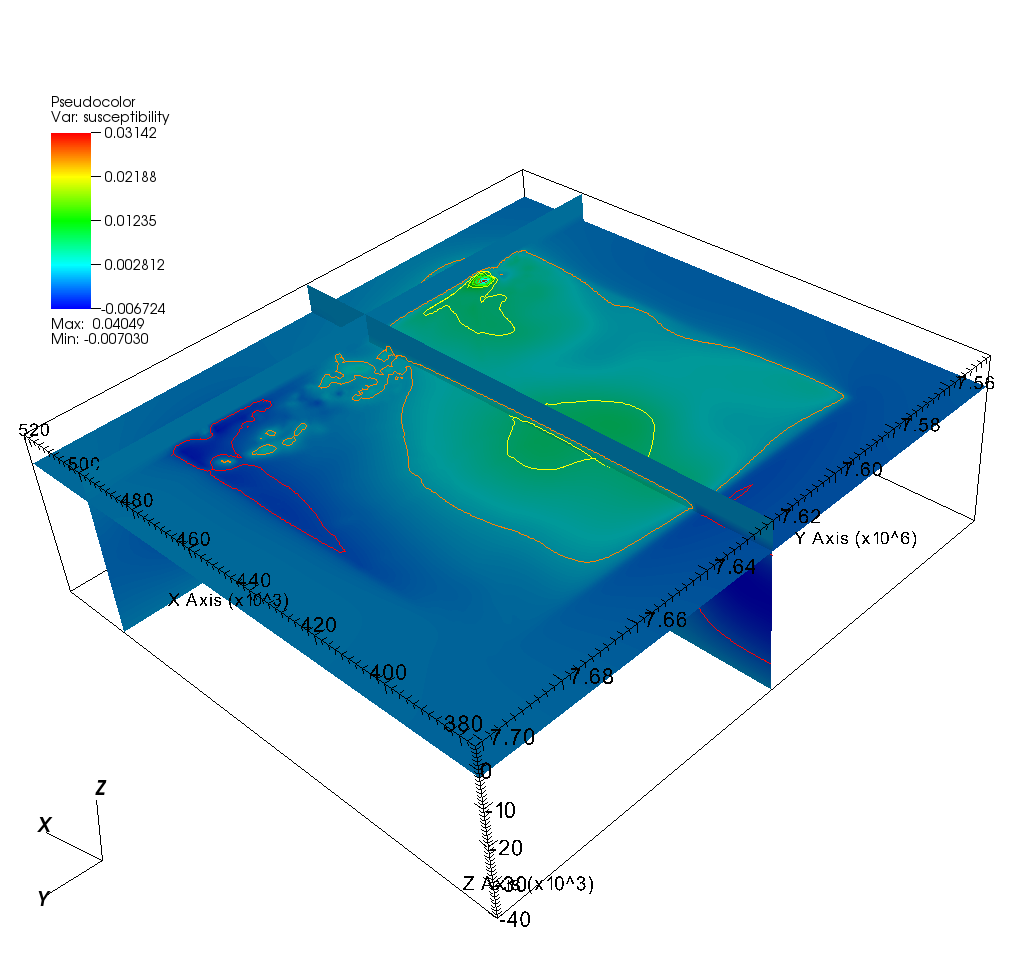
\includegraphics[width=\textwidth]{jointsus1.png}
% \caption{3D map on susceptibility result in joint inversion with two cross and a depth section}
% \label{fig:jointsus1}
% \end{figure}
% 
% \begin{figure}
% \centering
% 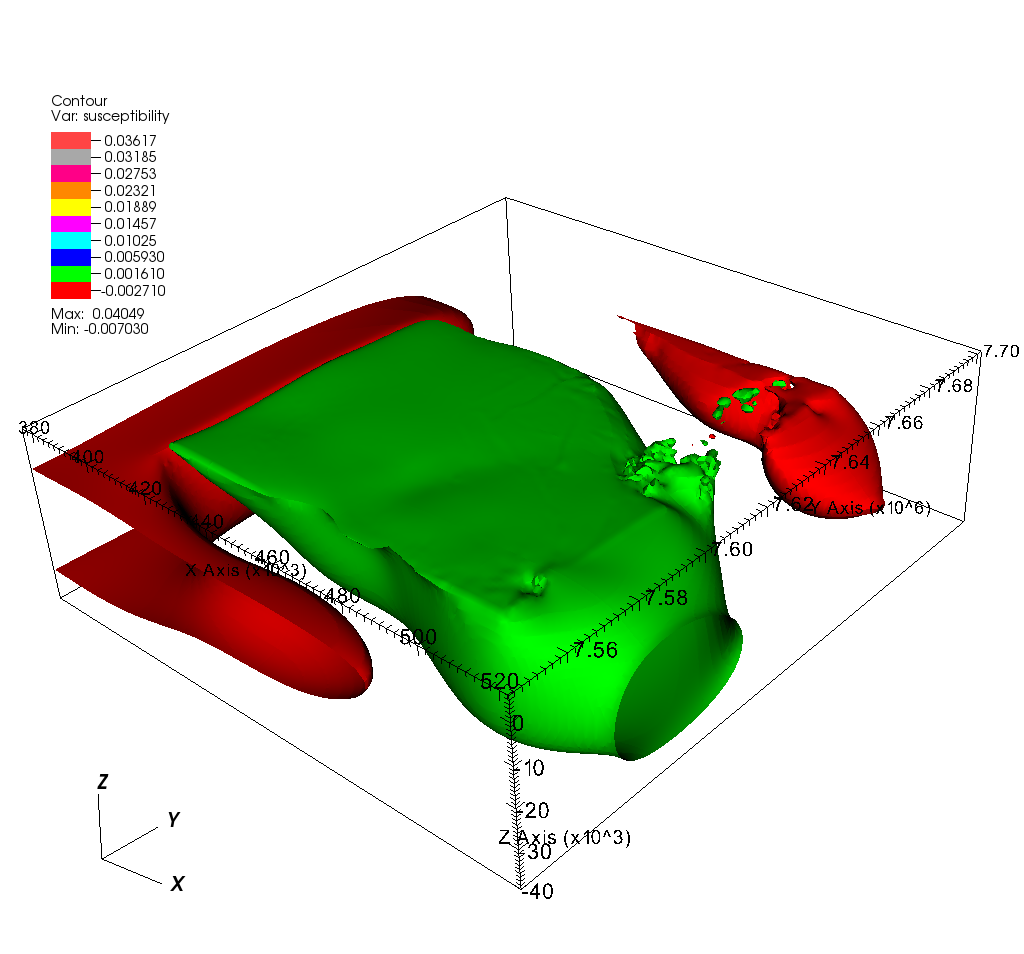
\includegraphics[width=\textwidth]{jointsus2.png}
% \caption{3D contour map on susceptibility result in joint inversion}
% \label{fig:jointsus2}
% \end{figure}


\section{Input File} 

According to the escript which is configured a prominent joint inversion in gravity and magnetic data, input data have contained gravity and magnetic anomalies data sets. In previous sections, gravity and magnetic data and their corrections, which need to invert, were distinguished in detail.

However it does not need to have data in one input file and they could be separately. It have to be mentioned that the inversion just run in the overlapping area with properly result.

Also its spacing is not important though the finer spacing , the better result. and its spacing could be differ in meter. 

Furthermore the script file for 2D and 3D inversion is apart and it have to be selected to have 2D or 3D inversion.

A small part of sample of inversion_gravmag_3d:

\begin{verbatim}
MAGNETIC_DATASET = 'mag.nc'
GRAVITY_DATASET = 'gravity.nc'
latitude = -28.5
PAD_X = 0.2
PAD_Y = 0.2
thickness = 40. * U.km
l_air = 6. * U.km
n_cells_v = 25
mu_gravity = 10.
mu_magnetic = 0.1
\end{verbatim}

Inversion_gravmag file consist many options to implement which control how joint inversion is performed such as padding area, depth , MU factor,\ldots. Which in previous section was explained in details. just some items are fixed for joint inversion such as mu.


\begin{description} 
\item[MAGNETIC_DATASET]In inversion_gravmag file the name of the magnetic file which contains the magnetic anomalies data should be defined.

\item[GRAVITY_DATASET]Because the gravity data is in another file, the name of the gravity file should be noted too.
	
\item[latitude]This is referred to the area of gathering data sets to calculate the main reference magnetic field. Which is selected -28 for east Australia.


\item[mu_gravity]It is defined in accordance with the noise of gravity data. and it is not the same as gravity inversion which is 10.

\item[mu_magnetic]It is determined as 0.1.

\end{description}


\section{Output File}

After preparing input files and submitting the 2D or 3D escript to run inversion, an output file will be created to show result of inversion. This file has silo extension and contains both density and susceptibility. Moreover it displays those values separately in a 2D or 3D model. The inversions dimension is related to our decision at the time of start up. Also its reference data is in output file to have a good comparison between output and input information.

% \section{Reference}
% 
% This is a 3D model as an example with three different density and two susceptibility humps in horizon which create nine density humps and four susceptibility humps in presented block. Two first images show the reference synthetic datasets (\ref{fig:joint3D4mag6grav-gref} and \ref{fig:joint3D4mag6grav-mref}) and two last images indicate result after joint inversion in two both magnetic and gravity.(\ref{fig:joint3D4mag6grav-g} and \ref{fig:joint3D4mag6grav-m})
%  
% \begin{verbatim}
% n_humps_h = 3
% n_humps_v = 1
% n_humpsm_h =2
% n_humpsm_v =1
% l_data = 100. * U.km
% mu=100
% \end{verbatim}
% 
% \begin{description} 	
% \item[n_humps_h]This is number of density humps in horizon of input file.
% 
% \item[n_humps_v]This is number of density humps in vertical of input file.
% 
% \item[n_humpsm_h]This is number of magnetic susceptibility humps in horizon of input file.
% 
% \item[n_humpsm_v]This is number of magnetic susceptibility humps in vertical of input file.
% 
% \item[l_data]The length of data is allocated to distribute data or humps.
% 
% \end{description}
% 
% 
% \begin{figure}
% \centering
% 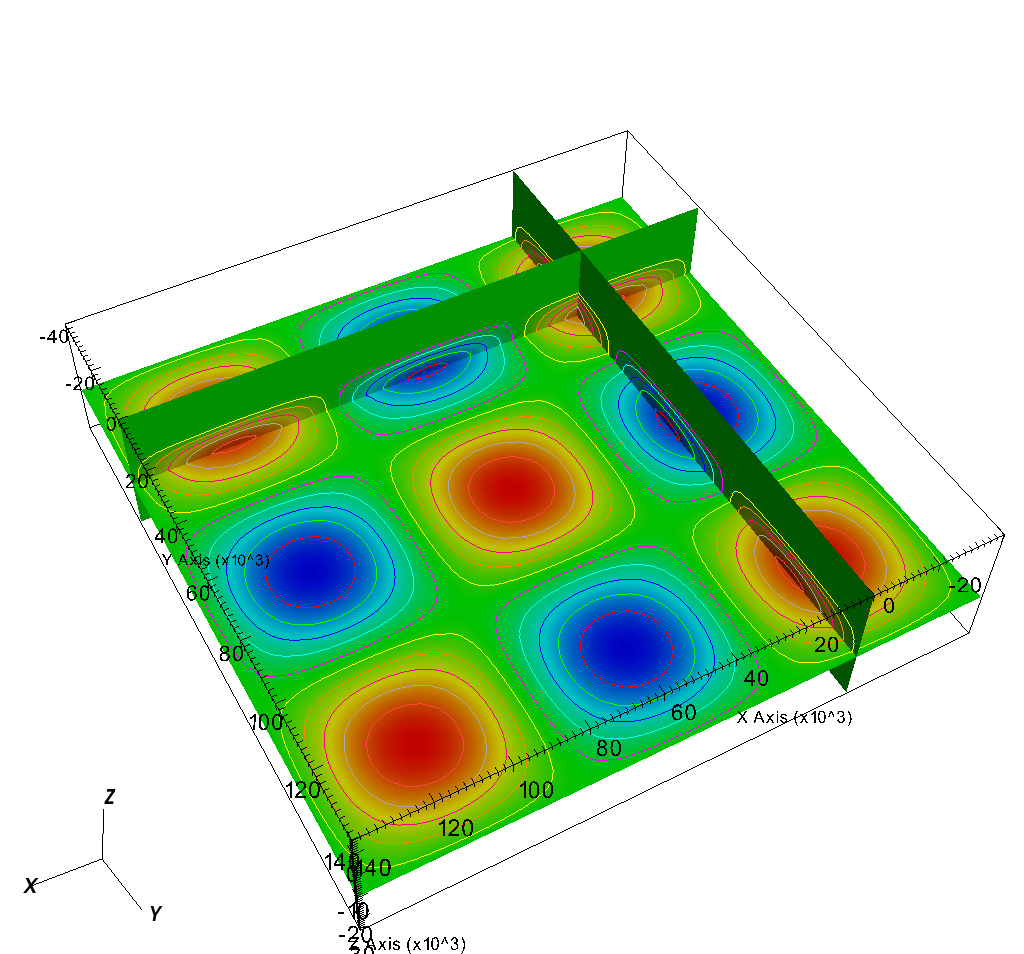
\includegraphics[width=\textwidth]{joint3D4mag6grav-gref.png}
% \caption{3D reference density model}
% \label{fig:joint3D4mag6grav-gref}
% \end{figure}
% 
% 
% \begin{figure}
% \centering
% 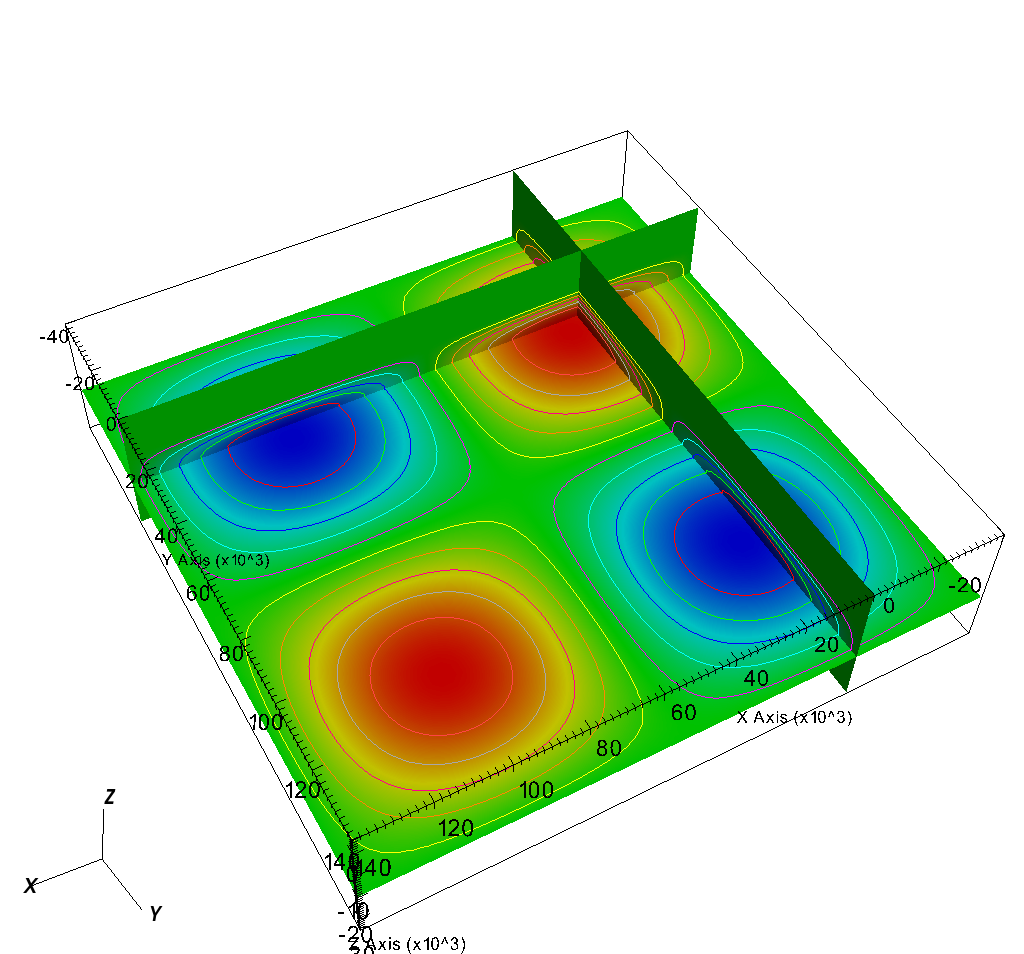
\includegraphics[width=\textwidth]{joint3D4mag6grav-mref.png}
% \caption{3D reference susceptibility model}
% \label{fig:joint3D4mag6grav-mref}
% \end{figure}
% 
% 
% \begin{figure}
% \centering
% 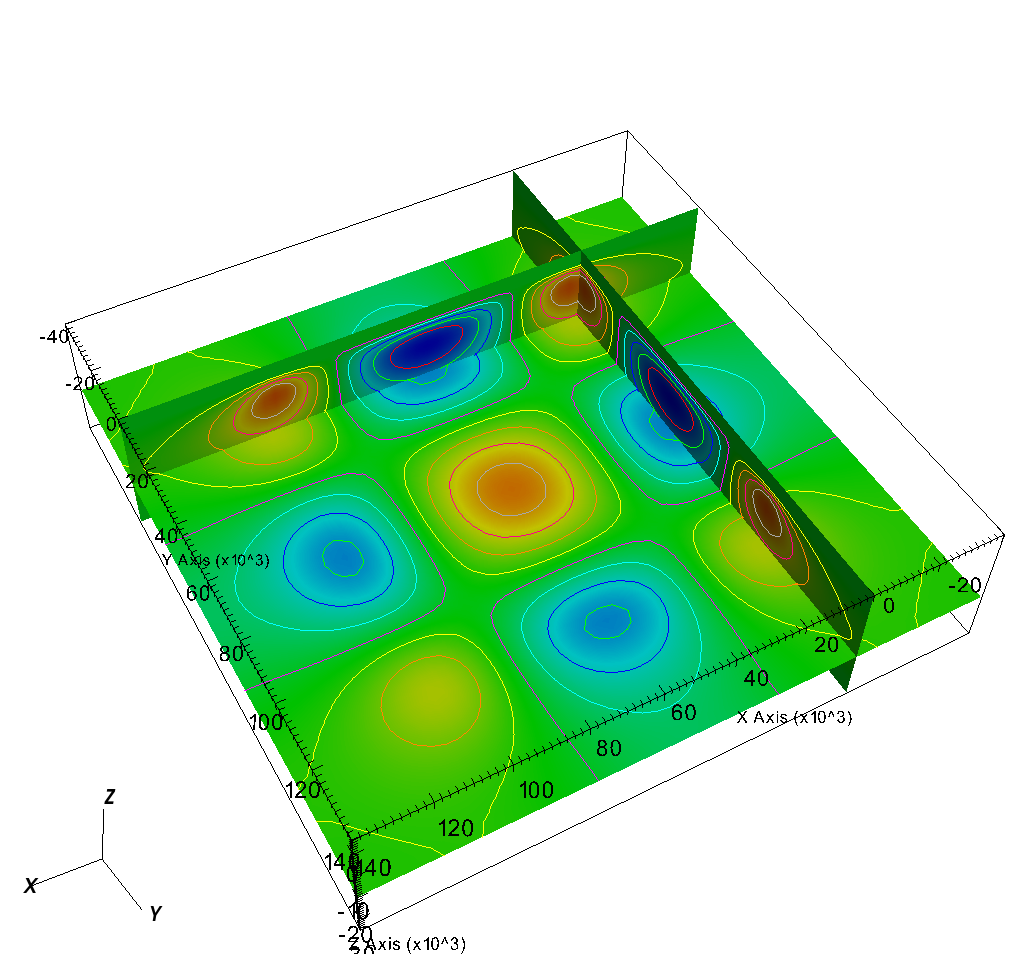
\includegraphics[width=\textwidth]{joint3D4mag6grav-g.png}
% \caption{3D result density model}
% \label{fig:joint3D4mag6grav-g}
% \end{figure}
% 
% 
% \begin{figure}
% \centering
% 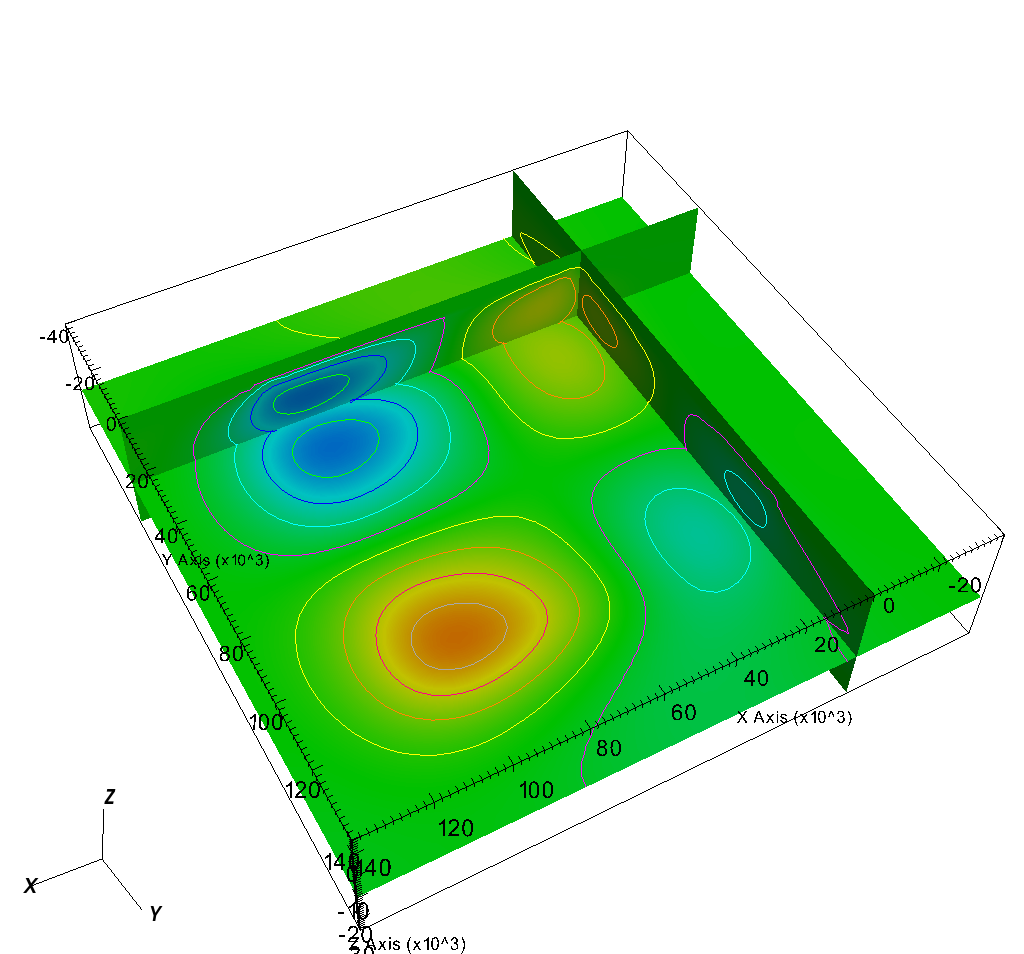
\includegraphics[width=\textwidth]{joint3D4mag6grav-m.png}
% \caption{3D result magnetic model}
% \label{fig:joint3D4mag6grav-m}
% \end{figure}
% 
